\documentclass{beamer}
\usepackage[T1]{fontenc}
\usepackage[english]{babel}
\usefonttheme{serif}
\setbeamertemplate{navigation symbols}{
\usebeamerfont{footline}
\usebeamercolor[fg]{footline}
\insertframenumber/\inserttotalframenumber{}
}
\setbeamerfont{frametitle}{size = \small}
\usepackage{mathpazo}
\usepackage{float}
\usepackage[labelsep = colon]{caption}
\usepackage{amsmath}
\usepackage{setspace}
\usepackage{graphicx}
\usepackage{threeparttablex}
\usepackage{longtable}
\usepackage{booktabs}
\usepackage{dcolumn}
\usepackage{pdfpages}


\title{GV217 Conflict Analysis, Week 21}
\subtitle{Causes of Conflict: Environmental}
\author{Muzhou Zhang\\ muzhou.zhang@essex.ac.uk\\ Virtual Office Hour: 15:30--16:30, Friday, 997 5800 8679}
\date{25 Feb 2022}

\begin{document}
\maketitle
\setstretch{1.25}

\begin{frame}{What Does Environmental Mean}
    \begin{itemize}
        \pause\item Long-term, systematic: climate
        \pause\item Short-term, idiosyncratic: weather\\
        \pause      But climate change causes more variable weather
        \pause\item The natural resources that people live with
        \pause      such as soils, forests, water, etc.
        \pause\item Environmental factors was auxiliary for causal inference for a longtime
    \end{itemize}
\end{frame}

\begin{frame}{Two Examples: Sino-Monadic Conflict}
    \pause
    \begin{center}
        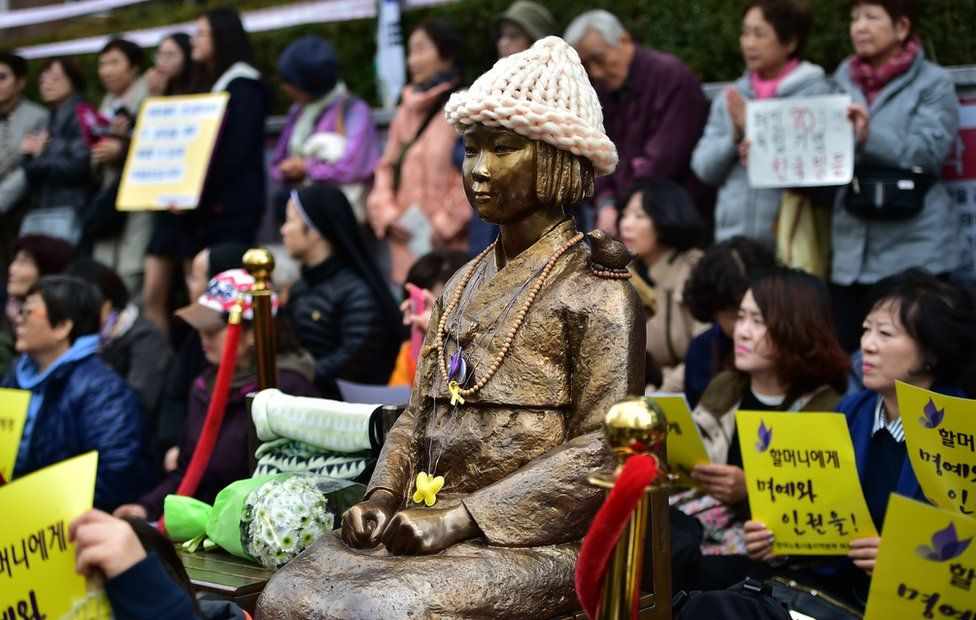
\includegraphics[width = \linewidth]{/Users/mz/Desktop/GitHub/teaching/gv217_conflict_analysis/figs/wk21/fig1.png}
    \end{center}
    \tiny Zhang et al. (2007, \emph{Human Ecology}); see also Bai \& Kung (2011, \emph{REStat})
\end{frame}

\begin{frame}{Two Examples: Sino-Monadic Conflict}
    \pause
    \begin{center}
        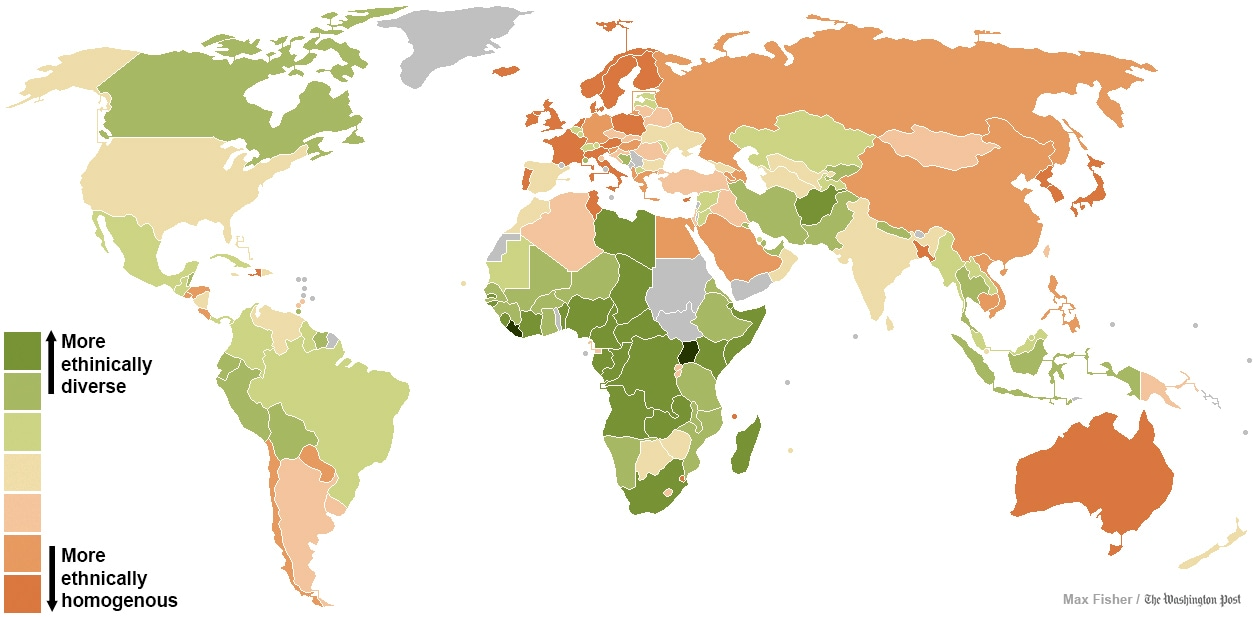
\includegraphics[height = 0.75\linewidth]{/Users/mz/Desktop/GitHub/teaching/gv217_conflict_analysis/figs/wk21/fig2.png}
    \end{center}
    \tiny Zhang et al. (2007, \emph{Human Ecology}); see also Bai \& Kung (2011, \emph{REStat})
\end{frame}

\begin{frame}{Two Examples: Syrian Civil War}
    \pause
    \begin{center}
        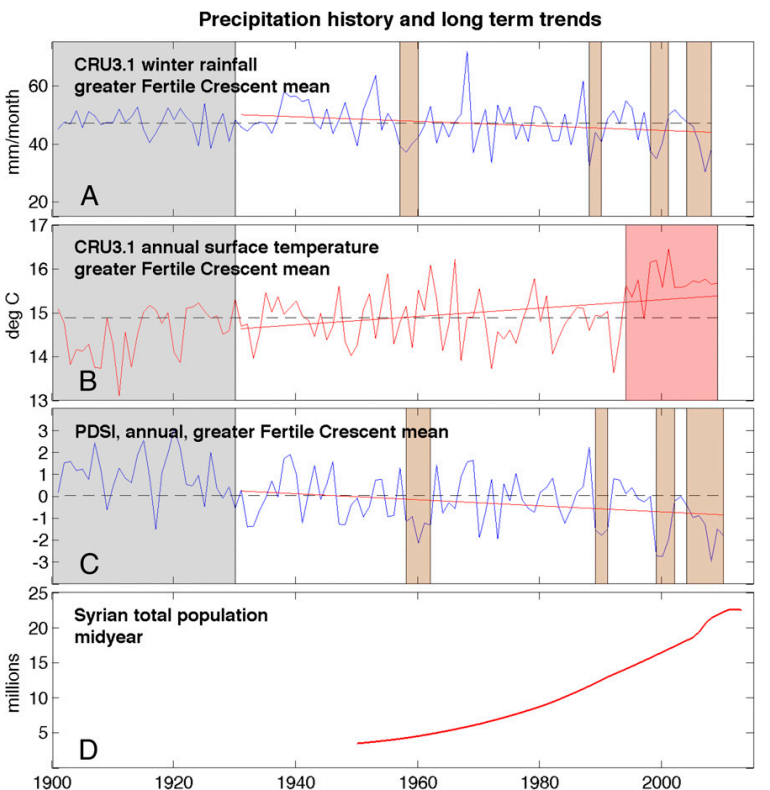
\includegraphics[height = 0.75\linewidth]{/Users/mz/Desktop/GitHub/teaching/gv217_conflict_analysis/figs/wk21/fig3.png}
    \end{center}
    \tiny Kelley et al. (2015, PNAS) 
\end{frame}

\begin{frame}{Two Examples: Syrian Civil War}
    \pause
    \begin{center}
        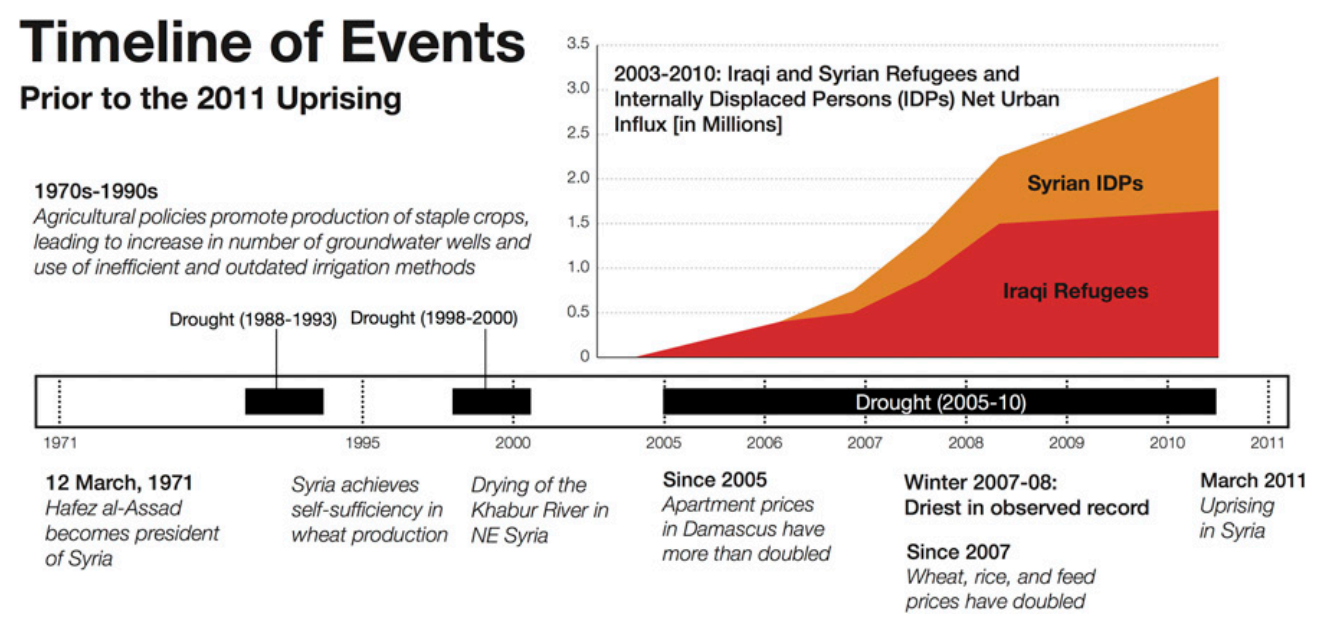
\includegraphics[width = \linewidth]{/Users/mz/Desktop/GitHub/teaching/gv217_conflict_analysis/figs/wk21/fig4.png}
    \end{center}
    \tiny Kelley et al. (2015, PNAS) 
\end{frame}

\begin{frame}{Why the Environment Matters}
    \pause
    \begin{center}
        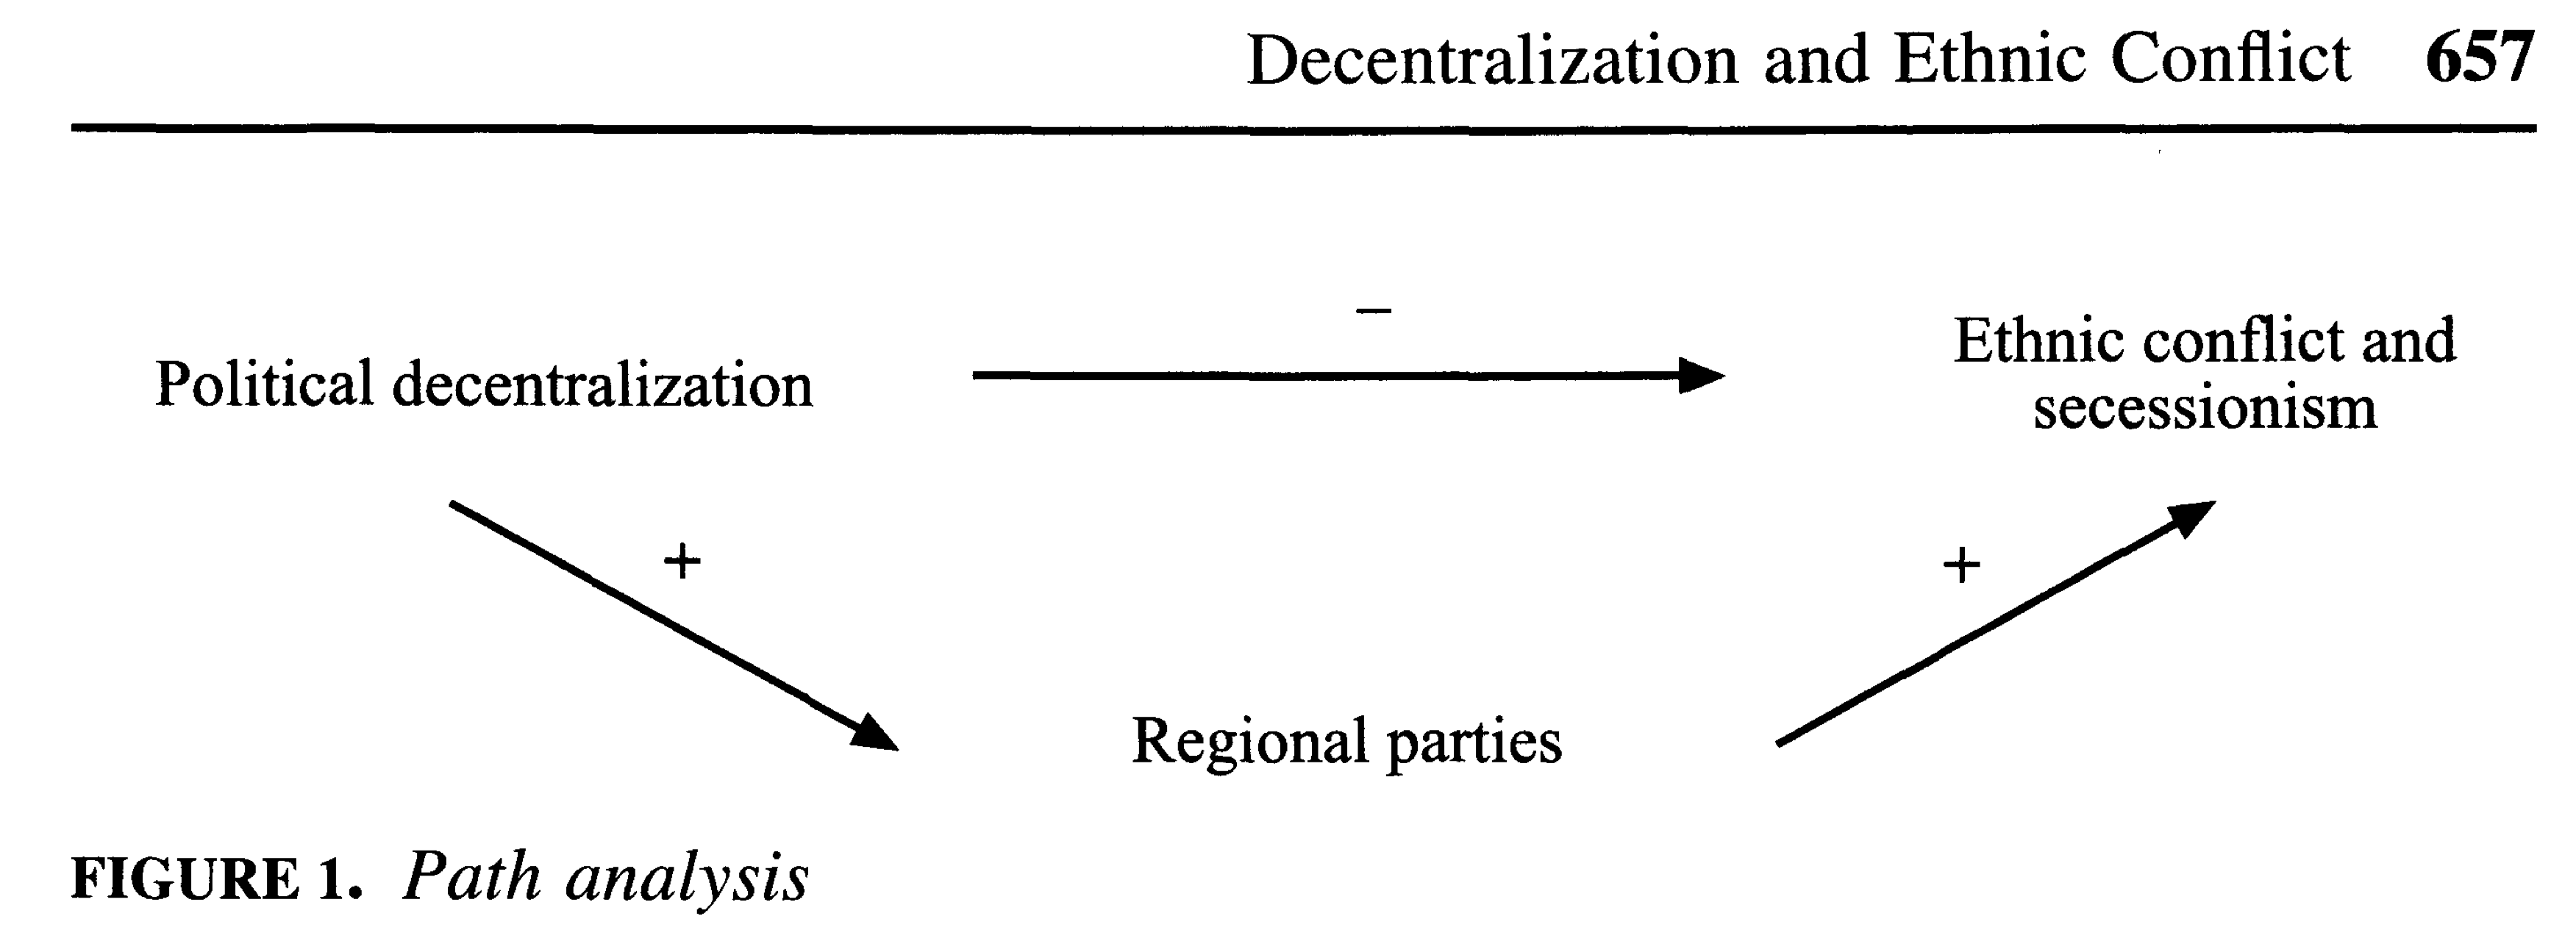
\includegraphics[width = \linewidth]{/Users/mz/Desktop/GitHub/teaching/gv217_conflict_analysis/figs/wk21/fig5.png}
    \end{center}
\end{frame}

\begin{frame}{Why the Environment Matters}
    \pause
    \begin{center}
        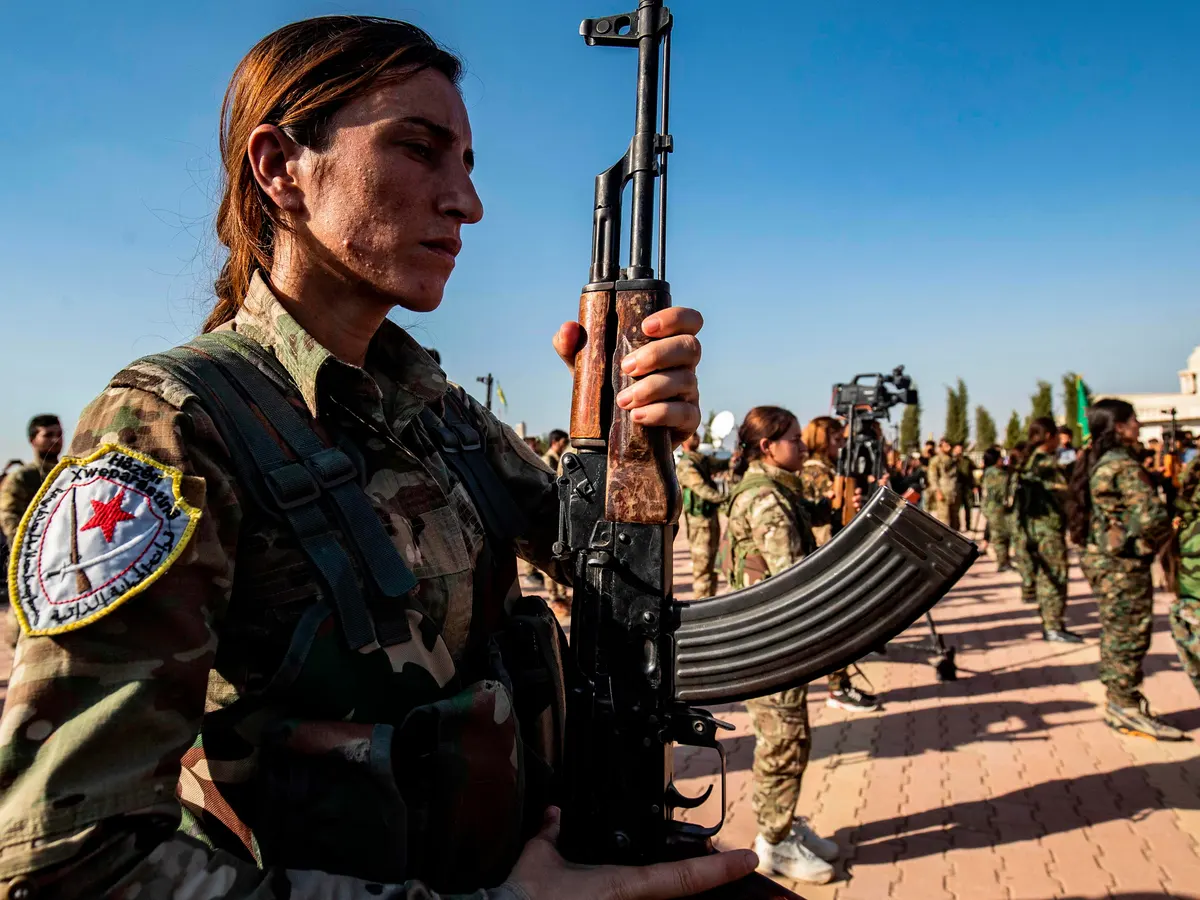
\includegraphics[width = \linewidth]{/Users/mz/Desktop/GitHub/teaching/gv217_conflict_analysis/figs/wk21/fig6.png}
    \end{center}
\end{frame}

\begin{frame}{Why the Environment Matters}
    \pause
    \begin{center}
        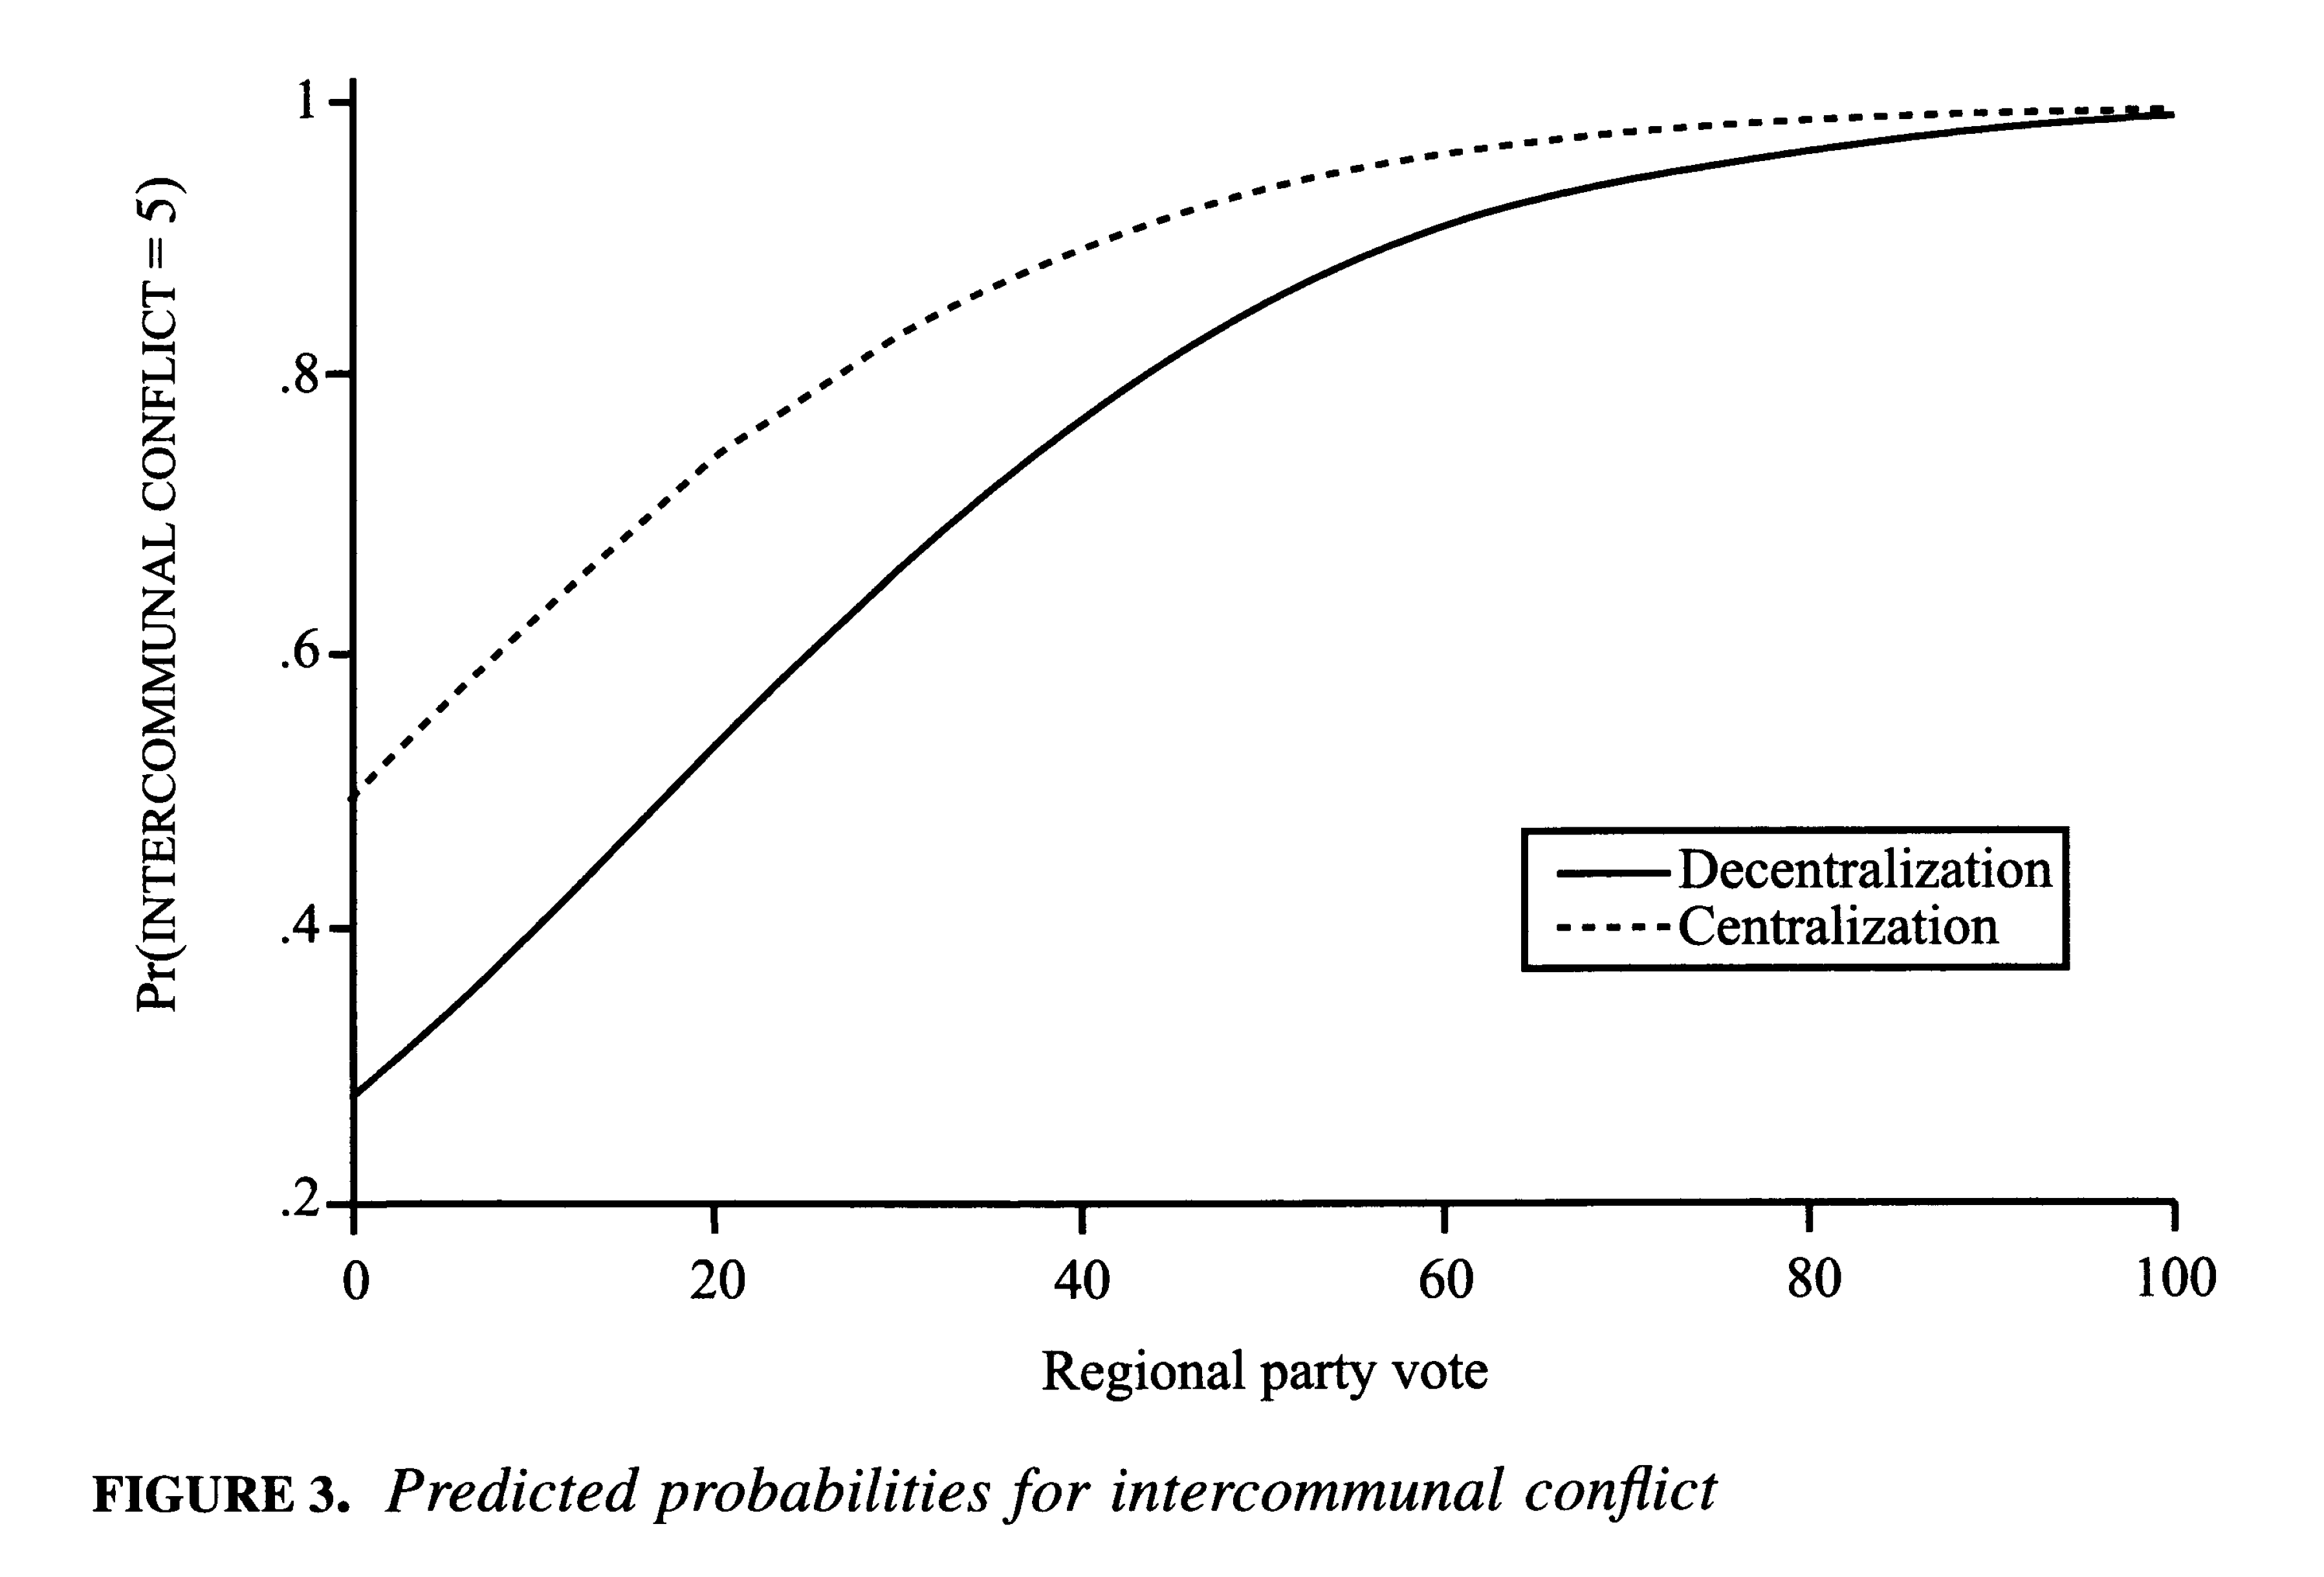
\includegraphics[width = \linewidth]{/Users/mz/Desktop/GitHub/teaching/gv217_conflict_analysis/figs/wk21/fig7.png}
    \end{center}
    \tiny © Verisk Maplecroft
\end{frame}

\begin{frame}{Why the Environment Matters}
    \pause
    \begin{center}
        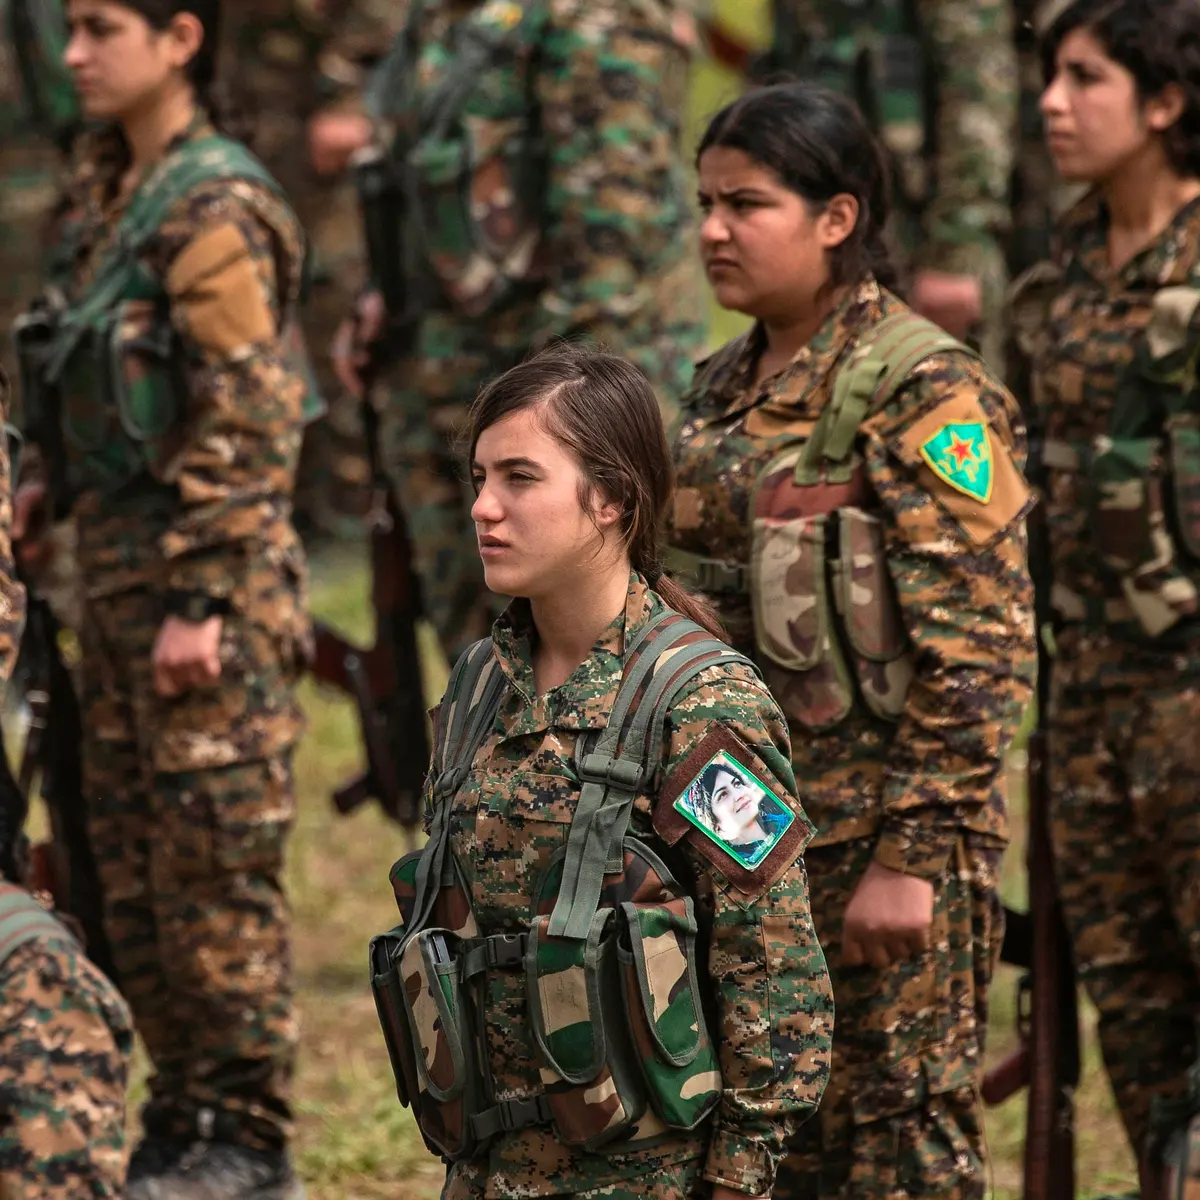
\includegraphics[width = \linewidth]{/Users/mz/Desktop/GitHub/teaching/gv217_conflict_analysis/figs/wk21/fig8.png}
    \end{center}
\end{frame}

\begin{frame}{Why the Environment Matters}
    \pause
    \begin{center}
        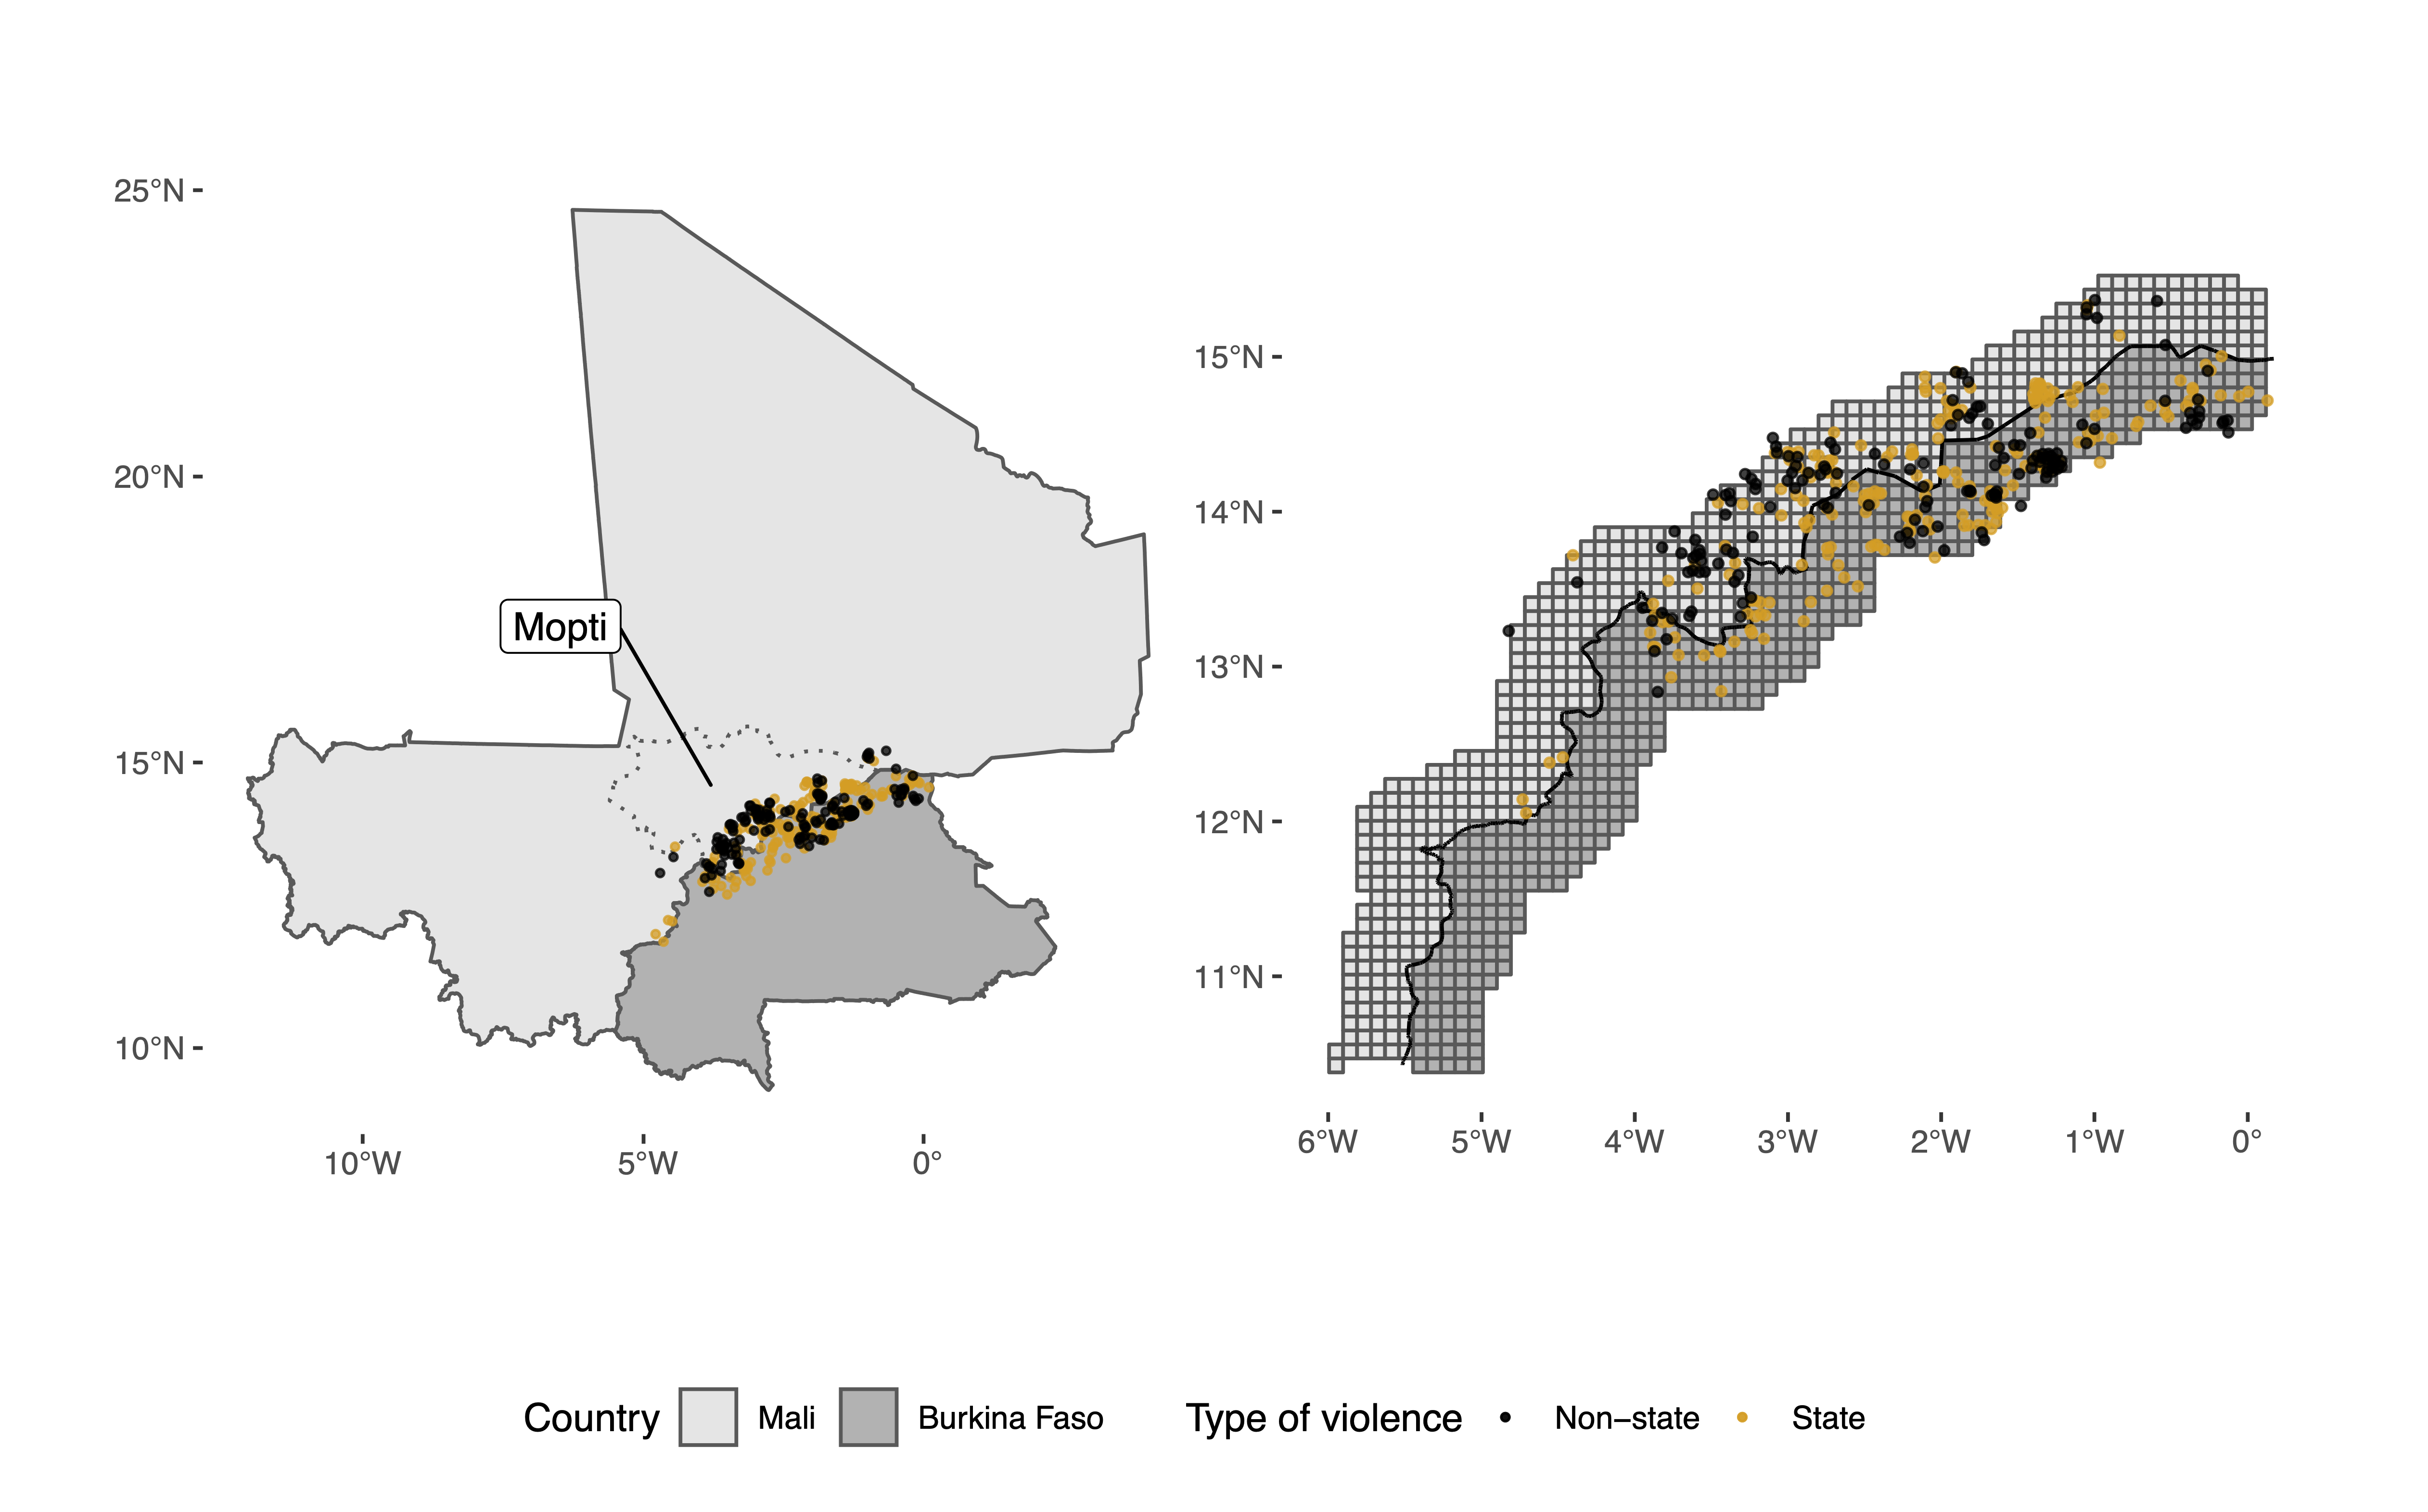
\includegraphics[height = 0.75\linewidth]{/Users/mz/Desktop/GitHub/teaching/gv217_conflict_analysis/figs/wk21/fig9.png}
    \end{center}
    \tiny Kikuta (2020, \emph{JOP})
\end{frame}

\begin{frame}{Two Questions}
    \begin{itemize}
        \pause\item Does positive anomaly have effect?\\
        \pause      See, for example, Landis (2014, \emph{JPR})
        \pause\item Are the findings causal?
    \end{itemize}
\end{frame}

\begin{frame}{Correlation Is Not Causation}
    \pause
    \begin{center}
        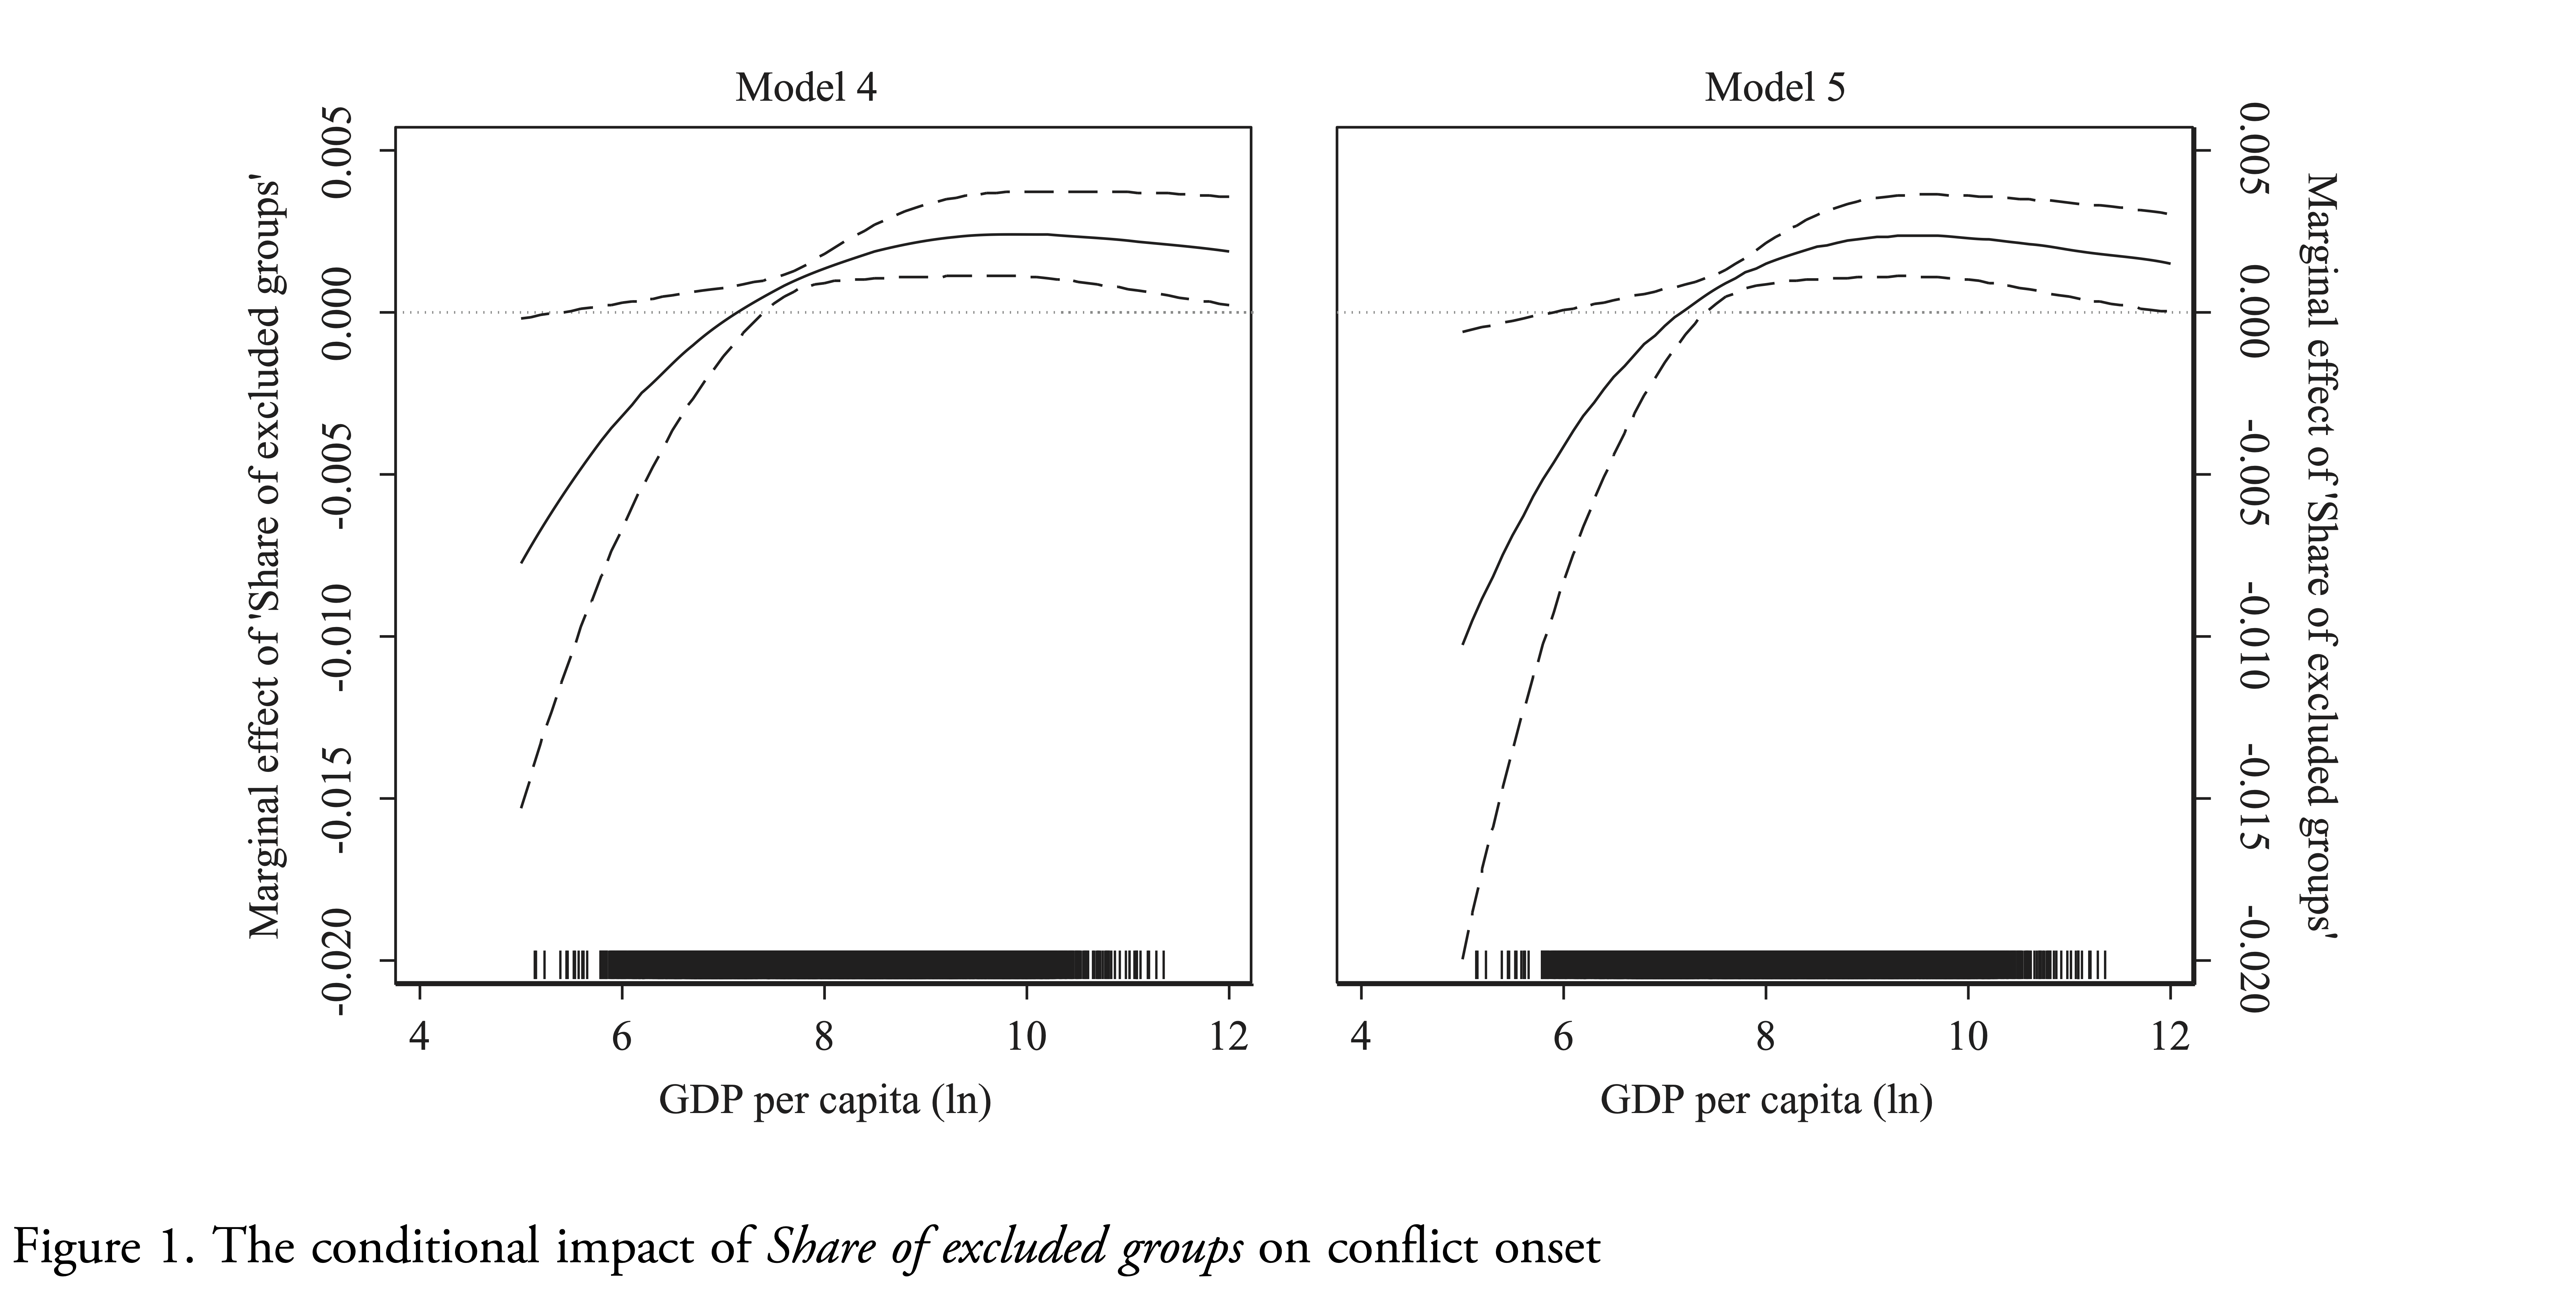
\includegraphics[width = \linewidth]{/Users/mz/Desktop/GitHub/teaching/gv217_conflict_analysis/figs/wk21/fig10.png}
    \end{center}
\end{frame}

\begin{frame}{Correlation Is Not Causation}
    \begin{itemize}
        \pause\item Potential outcome
        \pause\item The fundamental problem of causal inference
        \pause\item Counterfactuals
    \end{itemize}
\end{frame}

\end{document}